\begin{figure*}[t]
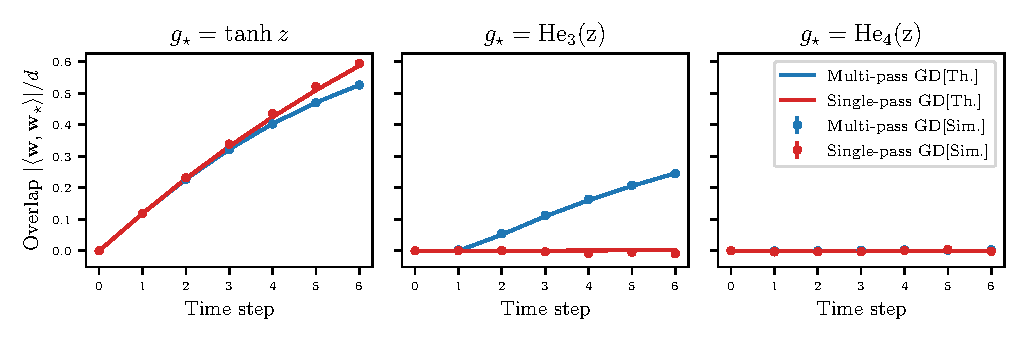
\includegraphics[width=0.95\textwidth]{figs/single_index_v2}
\vspace{-2em}
    \caption{\textbf{One-pass and multi-pass GD for single-index models --} The {\it overlap} $\left|\frac{\langle \vec w^\star,  \hat{\vec{w}}\rangle }{d}\right|$ between the learned weight and the target/teacher direction, is plotted as a function of the iteration time of both single-pass (red) and multi-pass (blue) GD.  Continuous lines are given theory,  dots are simulations. 
    \textbf{Left: Easy finite-T learnable single-index target} $g^\star \!=\! \tanh$: both one-pass and multi-pass GD obtain positive correlation after a finite number of iterations as the information exponent of the target is $\ell\!=\!1$.  \textbf{Center: Multi-pass finite-T learnable single-index target}: $g^\star \!=\! \mathrm{He}_3$. Multi-pass GD achieves a non-zero correlation in just two steps, but the one-pass algorithm learns nothing. 
    % Notice that the optimal overlap in this problem is negative as $\mathrm{He}_3$ has a negative coefficient in its linear term. 
    \textbf{Right: Finite-time nonlearnable single-index targets} $ g^\star \!=\! \mathrm{He}_4$; the target function is even and thus, as stated in Thm.~\ref{thm:main:2step_learning}, breaking this symmetry is hard in finite number of steps, resulting in a vanishing correlation with the teacher direction $\vec w^\star$ for both algorithms in any finite time. (Simulation are averaged over $32$ runs,     $d=5000$, with $\sigma = \rm relu$, $n=3d$, $p=1$, $\eta = 0.1$).
    % See details in Appendix~\ref*{sec:app:hyperparams}
    }
    \label{fig:main:single_index}
\end{figure*} 


\begin{figure*}[t]
    %\centering
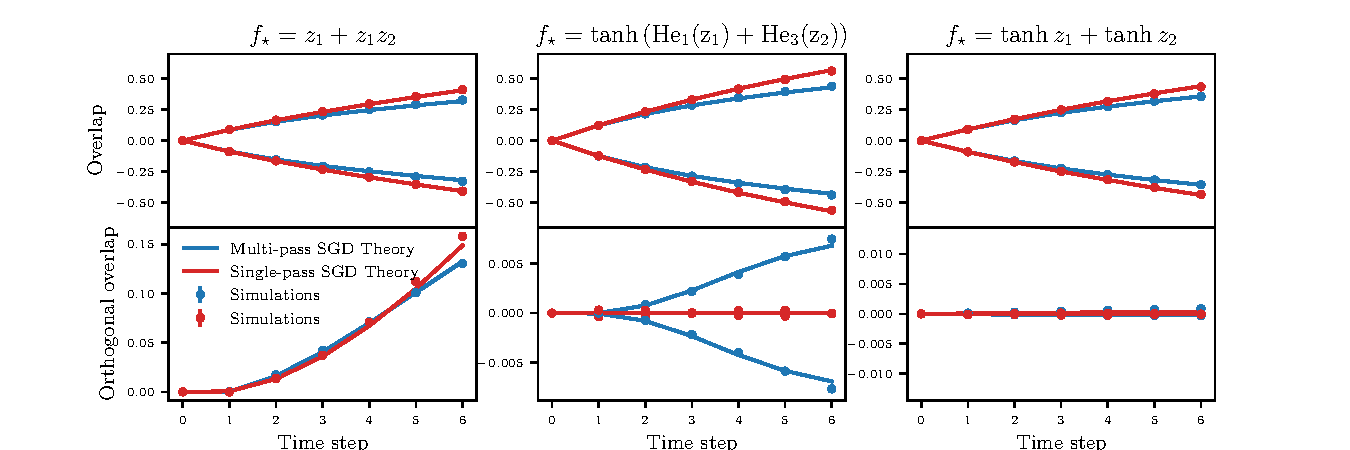
\includegraphics[width=1.05\textwidth]{figs/multi_index_v2}
\vspace{-2em}
    \caption{
    \textbf{One-pass and multi-pass GD for multi-index models --} 
The \textit{overlaps} between the student weights along the first direction learned, namely \(\mathbf{C}[f^\star]\), and its orthogonal, is plotted versus the number of iterations for three different classes of functions.     \textbf{Left: Easy finite-T learnable multi-index target} both the algorithms learn all the relevant directions when an "easy" function is used as a target (here (\(p=8\))).
     \textbf{Center: Multi-pass finite-T learnable multi-index target} both the algorithms learn the first Hermite direction \(\mathbf{C}[f^\star]\) but only multi-pass SGD achieve a non-null correlation in the orthogonal. This illustrates how reusing samples allows us to surpass the staircase limitation of single-pass approaches (\(p=2\)).
     \textbf{Right: Finite-time non-learnable multi-index target} neither of the two algorithm can learn \(\mathbf{C}[f^\star]^\bot\) with this target (\(p=2\)).
     (Simulation are averaged over $32$ runs,     $d\!=\!5000$, with $\sigma \!=\! \rm relu$, $n=3d$, $\eta \!=\! 0.1$).
    }
    \label{fig:main:multiple_index}
\end{figure*} 



\section{Statement of the results}
\label{sec:main:theory_results}
Here, we introduce the main results covering the theoretical learning guarantees with gradient descent and contrast them with the known one-pass results. We exploit the rigorous DMFT construction to prove the first key result: two-layer networks efficiently learn a large class of multi-index targets in only $T\!=\!2$ iterations, breaking the curse of one-pass algorithms dictated by the information and leap exponents. 
% \et{The iteration is also in Celentano, Montanari (although with a different proof)}



\subsection{Finite-T Learnable and Non-learnable directions}
We first identify which target directions are hard to learn for multi-pass gradient descent. Define $U^\star$ to be the subspace spanned by the rows of the target weights $W^\star$. The ``hard" directions are the ones where any transformation of the output $f^\star(\vec{z})$ does not lead to a linear correlation along the direction. 
We now define the subspace of such directions:


\begin{definition}\label{def:two_step_hard}
    We define $P^\star$ as the subspace of directions $\vec{v}^\star\in U^\star$ such that for any polynomial $F:\R \rightarrow \R$ with coefficients in $\R$, the following condition is satisfied:
    \begin{equation}\label{eq:f_hard_gen}
        \Eb{\vec{z}}{F(f^\star(\vec{z}))\langle \vec{v}^\star, \vec{z}\rangle}=0,
    \end{equation}
   % {\color{red}Fix the brackets in that equation.}
    Similarly, we denote by $A^\star$, the subspace of directions where the above condition is satisfied for all real-valued analytic functions $F$.
    % for $F=F_{\sigma, \vec{a}}$. Here $F_{\sigma, a}$ depends on the activation function $\sigma$ and the second layer $\vec{a}$, and is precisely defined in Appendix \ref{app:sec:main_thm_proof}. {\color {blue} Si}{\color{red}LZ: Can we define this $F_{\sigma, a}$ here?} 
    %   {\color{green}FK: This should be true for any function F, maybe we shoudl say this?}
    %   \et{Is it really ANY function? For sure it's a large class of function parametrised by $\sigma, a$, but I am not sure it's really ANY functions}
\end{definition}
One part of our main result shows that directions in $A^\star$ cannot be learned even by re-using batches of size $\cO(d)$ in a finite number of gradient steps. Furthermore, under suitable conditions on $\sigma$ and $\vec{a}$ (discussed in Theorem \ref{thm:main:2step_learning} and Appendix \ref{app:sec:main_thm_proof}), we show that after two gradient steps, the first layer learns all directions in the complement $P^\star_\perp$. We are now ready to state our main result: 

\begin{theorem}
\label{thm:main:2step_learning}
 Suppose that $n/d=\alpha>0$. Let $\vec{v}^\star\in P^\star_\perp$ denote an arbitrary direction in the orthogonal complement of the subspace $P^\star$ defined in definition \ref{def:two_step_hard} with norm $\sqrt{d}$ and a fixed representation in the basis $W^\star$.
Suppose further that the activation function $\sigma$ is analytic, with polynomially bounded derivatives satisfying $\Eb{z \sim \mathcal{N}(0,1)}{\sigma'(z)} \neq 0$ and $\sigma^k(0) \neq 0  \ \forall k \in \N$. Then, for any $g^\star$ with derivatives bounded by polynomials, there exist $\eta> 0, \lambda > 0$ such that almost surely over the choice of $\vec{a}$, we have:
\begin{equation}
    \norm{\frac{\vec{W}^{(2)}\vec v^\star}{d}} = \Theta_d(1) \,,
\end{equation}
with high probability as $n,d \rightarrow \infty$. Furthermore, for large enough $p$, $\vec{W}^{(2)}$ asymptotically spans $P^\star_\perp$:
\begin{equation}
    \inf_{\vec v^\star \in P^\star_\perp}\norm{\frac{\vec{W}^{(2)}\vec v^\star}{d}} = \Theta_d(1)\,,
\end{equation}
with high probability as $n,d \rightarrow \infty$.
In other words, directions $\vec v^\star \in P^\star_\perp$ are learned in $T=2$ gradient steps.  

Suppose, however that the teacher subspace $U^\star\!=\!A^\star$, then:
\begin{equation}
    \sup_{\vec v^\star \in U^\star} \norm{\frac{\vec{W}^{(t)} \vec v^\star}{d}} = o_d(1)\,,
\end{equation}
with high probability as $n,d\! \rightarrow\! \infty$, for any finite time $t$. Thus, none of the directions are learned in any finite number of GD steps.\looseness=-1
\end{theorem}
The proof is based on the analysis of the DMFT equations discussed
in Sec. \ref{sec:main:asymptotics}, is given in App.~\ref{sec:app:proofs}, and we provide an informal heuristic derivation in sec. \ref{sec:hidden_prog}.
While the above negative result requires all directions in $U^\star$  to be in $A^\star$ and thus in $P^\star$, in App \ref{sec:app:staircase}, we discuss the more general setup where learning of certain directions in $P^\star_\perp$ can affect the learning of directions in $U^\star$ in subsequent timesteps.

When the expectation in Equation \ref{eq:f_hard_gen} is non-zero for $F$ being the identity mapping, i.e. $F = \mathrm{id}$, $\vec{v}^\star$ is in-fact learned in the first gradient step \citep{ba2022high,dandi2023how} or through online SGD \citep{arous2022high,abbe2023sgd}. We discuss this further in Section \ref{sec:com_multi_vs_once}.

Our analysis reveals that the effect of re-using batches is to implicitly transform the output in the subsequent steps, allowing a larger set of directions to be learned. However, for directions in $A^\star$, such transformations are still insufficient.

\subsection{Characterization of hard directions through symmetries}

While Definition \ref{def:two_step_hard} characterizes the subspace of hard directions 
$A^\star$, it requires checking that the equality in Equation \ref{eq:f_hard_gen} holds for any real analytic transformation $F$.
We now show that a sufficient condition for $\vec{v}^\star \in A^\star$ is for $f^\star$ to possess certain symmetries along  $\vec{v}^\star$. This leads us to identify subspaces of hard directions, contained in $A^\star$, linked to symmetries w.r.t certain transformations. We characterize such subspaces below. The simplest such symmetry is defined through reflection along $\vec{v}^\star$:

\begin{definition}\label{def:symmetric_subspace}
   For any direction $\vec{v}^\star \neq 0 \in \R^d$, let $R_{\vec{v}^\star}$ denote the reflection operator along $\vec{v}^\star$, i.e. $R_{\vec{v}^\star}=\vec{I}-2\frac{1}{\norm{\vec v^\star}^2}\vec{v^\star}\vec{v^\star}^T$. We say that a direction $\vec{v}^\star \in U^\star$ is \text{even-symmetric} w.r.t $f^\star$ if for any $\vec{z} \in \R^d$:
    \begin{equation}
        f^\star(R_{\vec{v}^\star}\vec{z})= f^\star(\vec{z})
    \end{equation}
    We denote by $E^\star$ the subspace spanned by all \text{even-symmetric} directions in $U^\star$.
\end{definition} 
It is straightforward to see that any $\vec{v}^\star \in E^\star$ leads to Equation \ref{eq:f_hard_gen} being satisfied for any transformation $F$, since $\vec{v}^\star$ remains even w.r.t the function $F\left(f^\star (\cdot)\right)$. Therefore, $E^\star \subseteq A^\star$
However, the set of non-learnable directions can be larger due to the presence of additional symmetries. We now define such a larger subspace of hard directions arising due to a symmetry w.r.t reflections along $\vec{v}^\star$ coupled with orthogonal transformations along the orthogonal subspace:

\begin{definition}\label{def:ortho_symmetric_subspace}
   For any direction $\vec{v}^\star \neq 0$ in $U^\star$, let $R_{\vec{v}^\star}$ be as defined in Definition \ref{def:symmetric_subspace}. Let $O_{\perp}$ be a matrix in the orthogonal group on the $d-1$ dimensional subspace $\{\vec v^\star\}_\perp$ i.e the orthogonal complement of the linear subspace spanned by $\vec{v}^\star$.
        We say that a direction $\vec{v}^\star$ is \text{orthogonally-even-symmetric} w.r.t $f^\star$, if there exists an $O_{\perp} \in O(\{v^\star\}_\perp)$, such that for any $\vec{z} \in \R^d$:
    \begin{equation}
        f^\star(O_{\perp}R_{\vec{v}^\star} \vec{z})= f^\star(\vec{z})
    \end{equation}
    We denote by $OE^\star$ the subspace spanned by all \text{orthogonally-even-symmetric} directions in $U^\star$.
\end{definition} 

By setting $O_{\perp}$ as the identity mapping in the above definition, we recover the condition for $\vec{v}^\star \in E^\star$. Therefore, we have that $E^\star \subseteq OE^\star$.
While $OE^\star$ is the largest set of directions we've identified as being hard, the true set of hard directions may be larger still and is given by $A^\star$ in Definition \ref{def:two_step_hard}. We show in Appendix \ref{app:sec:proof:OE} that the directions in $OE^\star$ are indeed hard as per Definition \ref{def:two_step_hard}:
\begin{proposition}\label{prop:OE}
Let the subspaces $A^\star$ and $OE^\star$  be as defined in Defs. \ref{def:two_step_hard} and \ref{def:ortho_symmetric_subspace} respectively. Then, $OE^\star \subseteq A^\star$ i.e. all directions in $E^\star, OE^\star$ are hard as per Thm. \ref{thm:main:2step_learning}.
\end{proposition}

App.\ref{sec:app:even_sym} gives several examples  where $P^\star_\perp = E_\perp^\star = U^\star$, such as single-index targets with odd Hermite activations, staircase functions, etc.
Interestingly, we show that there exist functions $f^\star$ where the set $OE^\star$ is strictly larger than $E^\star$. Consequently, for such functions, $E^\star$ is strictly contained in  $A^\star,P^\star$. We discuss such target functions in Appendix \ref{sec:app:hard_sym}.
 For example, we show in Appendix \ref{sec:app:hard_sym}, that for the target function $f^\star(\vec{z})= z_1z_2z_3$, the direction $\vec{v}^\star=\vec{e}_1+\vec{e}_2+\vec{e}_3$ does not lie in $E^\star$ but lies in $OE^\star$ and thus in $A^\star,P^\star$.
 \vspace{-0.2cm}

 % In Appendix \ref{sec:app:hard_sym}, we provide additional examples of such directions not belonging to $E^\star$. {\color{red}LZ: This last paragraph is still not clear!!! First of all shall we make a 3rd definition where for any F the expectation is zero? Do we formally show this leads to finite-T hardness? }
%We refer to next section for the illustration of typical instances of the above subspaces in different scenarios. 

%Let us now give representative examples for which the above theorem apply \lp{these examples are going to be incorporated in the next section 3.2}: 
%\begin{itemize}[noitemsep,leftmargin=1em,wide=0pt]
 %   \item \textbf{Symmetric functions:} Let the teacher be $f_\star(\vec z) = g_\star (\langle \vec \theta_*, \vec z \rangle)$ with $g_\star$ even function. In this case the subspace $E^\star$ is the full teacher subspace $U^\star$, hence no direction is learned in finite number of steps by multi-pass GD.
  %  Specializing to the phase retrieval case, i.e. $g_\star(\cdot) = (\cdot)^2 $, we recover well-known behaviour where iterative algorithms do not learn this function in a finite number of steps \citep{maillard2020phase}.
    %
    %\item \textbf{Non-symmetric functions:} By removing the parity assumption on $g_\star(\cdot)$, the set $E^\star$ becomes empty and multi-pass GD learns $\vec \theta_\star$ in just $T=2$ steps. 
    
%    \item \textbf{Commitee machines:} Let the target be: $f_\star(\vec z) = \frac{1}{k} \sum_{r=1}^k \sigma_r (\langle \vec \theta_\star^r, \vec z \rangle)$. This class of \textit{commitee targets} has been characterized to present computational barriers, e.g. \citep{aubin2020generalization}. Indeed, if we take $\sigma_r = \sigma_{r^\prime}$, upon permutation between neurons, the only relevant non-even direction will be $\sum_{r}\theta_\star^r$. Our results imply that multi-pass GD learns only the best single-index approximation of the committee target from $O(d)$ samples in finite time.  Conversely, if $\sigma_r \neq \sigma_{r^\prime}$ for all pairs $r,r^\prime$, the exchange symmetry is lost, and the hidden units of the two-layer network learn after $T=2$ GD steps on the same batch. 
%\end{itemize}

%\subsection{Breaking the curse of information and leap exponents}
\subsection{Comparison between one-pass and multi-pass GD}\label{sec:com_multi_vs_once}

%{\bf Maybe this could be later? We can give examples for all three caterories?}

Our results are particularly interesting in the context of a recent line of work on the limitations of one-pass algorithms. 
%The characterization of functions that are hard to learn for one-pass GD was established in a considerable number of works 
\citep{arous2021online,abbe2021staircase,abbe2022merged,abbe2023sgd,dandi2023how,bietti2023learning,zweig2023symmetric}. We can demonstrate, in particular, a sharp separation performance between one-pass and multiple-pass protocols.

\paragraph{Learning single-index targets --} 
First, we consider single index targets.
%In this class of functions, 
Targets that are hard to learn 
%the settings which are hard to learn 
for one-pass algorithms starting from uninformed initialization in high dimension are characterized by the \textit{Information Exponent} ($\rm{IE}$). Informally, the $\rm{IE}$ is equivalent to the first non-zero coefficient in the Hermite expansion of the target activation. 
\begin{definition}[Information Exponent]
\label{def:main:information_exponent}
\citep{arous2021online}
Let $\mathrm{He}_j$ be the $j-$th Hermite polynomial. Using the definition for the target of eq.~\eqref{eq:main:teacher_def},  reading in the single-index case as $f^\star = g^\star(\langle \vec w^\star, \vec z \rangle)$,  the $\rm IE$ is defined as:
\begin{align}
{\rm{IE}} = \min \{j\in\mathbb{N}: \mathbb{E}_{\xi \sim \mathcal{N}(0,1)} \left[g^{\star}(\xi) \mathrm{He}_j(\xi)  \right]\neq 0\} 
\end{align}
\end{definition}
Higher $\rm IEs$ are associated to harder problems for one-pass training protocols. Indeed, \citep{arous2021online} provably show that one-pass SGD, with one sample per batch, weakly recovers the teacher direction $\vec w^\star$ only upon iterating the training schedule for $T(\rm IE)$ time iterations:
% LP: greedy solution using \hspace because I would like to avoid as many external packages as possible (desk-reject iclr) and the stack overflow solution suggest them. I will fix this
\begin{align}
\label{eq:main:time_complexity_IE}
    T(\rm IE) = \begin{cases}
        &\cO(d^{\rm IE -1} ) \qquad \hspace{0.3em}\text{if $\rm{IE}>2$} \\
        &\cO(d \log{d} ) \qquad \text{if $\rm{IE}=2$} \\
        &\cO(d) \qquad \hspace{2.2em}\text{if $\rm{IE}=1$}
    \end{cases}
\end{align}
Recently, the time complexity has been improved up to the Correlational Statistical Query (CSQ) lower bound of $d^{\max{(\frac{\rm{IE}}{2}},1)}$, by considering an appropriate smoothing of the loss \citep{damian2023smoothing}.
Definition~\ref{def:main:information_exponent} has been extended to larger batch sizes in \citep{abbe2022merged,dandi2023how}, without changing the overall picture; more precisely, even with $n = o(d^{\rm{IE}})$ fresh samples per batch, one-pass training procedures are still not able to weakly recover the signal in finite iteration time. The case $\rm IE=1$ corresponds to the expectation in Equation \ref{eq:f_hard_gen} being non-zero for $F=\mathrm{id}$. However, since Definition \ref{def:two_step_hard} allows for general transformations $F$ to the output $f^\star$, $\vec{w}^\star$ may not be in $P^\star, A^\star$ even when $\rm{IE} > 1$. The presence of general transformations $F$ in definition \ref{def:two_step_hard} allows our algorithm to bypass CSQ bounds, which are restricted to $F=\mathrm{id}$. Such general transformations are however permitted under the framework of Statistical Query (SQ) algorithms \citep{kearns1998efficient}. We thus expect gradient descent with  $\cO(d)$ sample complexity to inherit the hardness results established for the class of SQ algorithms \citep{diakonikolas2020algorithms,goel2020superpolynomial,chen2021efficiently,chen2022hardness}.
We emphasize however that unlike explicit SQ algorithms, our analysis shows that gradient descent performs such transformations implicitly, allowing it to reach the optimal complexity of SQ algorithms for certain class of target functions.
\looseness=-1

We illustrate the sharp contrast between one-pass and multiple-pass protocols with the examples depicted in Figure~\ref{fig:main:single_index}, which shows the scalar product (called \textit{overlap}) between the learned weights and the teacher direction as a function of the time steps and compares simulation (dots) with theoretical predictions (continuous lines). There are $3$ cases:
\vspace{-0.3cm}
\begin{itemize}[noitemsep,leftmargin=1em,wide=0pt]
    \item \textbf{Easy finite-$T$ learnable single-index targets $\left(\rm{IE}\!=\!1\right)$:} The left panel of Fig.~\ref{fig:main:single_index} show the learning curve for a problem with $\rm{IE} \!=\! 1$. {\it Both} single-pass and multiple-pass GD correlates with the target in finite time. The non-symmetric subspace coincides with the teacher one $E_\perp^\star = U^\star$ (Def.~\ref{def:symmetric_subspace}).
    \item \textbf{Multi-pass finite-$T$ learnable single-index targets $\left(\rm IE\!>\!1, \rm {non-even \,\,f^\star} \right)$: }  Fig.~\ref{fig:main:single_index} (center) depicts the learning curve for a non-even target function, with $\rm{IE} = 3$. Here, one-pass GD is not able to achieve any significant correlation with the teacher $\vec w^\star$ (and it would require a number of iterations $T = \cO(d)$ to achieve weak recovery - see eq.~\eqref{eq:main:time_complexity_IE}). However, multiple-pass GD performs weak recovery in only $T=2$ steps. As before, the non-symmetric subspace corresponds to the teacher one $E_\perp^\star = U^\star$ (Def.~\ref{def:symmetric_subspace}).
    \item \textbf{Finite-$T$ non-learnable single-index targets $\left(\rm{IE}\!>\!1, \, \, even \,\, f^\star\right)$:} Fig.~\ref{fig:main:single_index} (right) considers an even problem, with $\rm IE = 4$. Neither of the training procedures achieve weak recovery  in finite time. The computational hardness of this problem is associated with the presence of symmetry in the teacher function that requires time to break. Indeed, following Definition~\ref{def:symmetric_subspace}, the even-symmetric subspace $E^\star$ is equivalent to the teacher subspace $U^\star$. These results agree with the emergence of \textit{computational barriers } in symmetric single-index problems like the phase retrieval one \citep{maillard2020phase}. In fact, for such problems, regardless of the number of iterations, learnability requires $\alpha$ to be larger than critical values even for the most efficient known algorithms (see \citep{barbier2019optimal}, Sec. 3.1).
    % \item  \dots If the non-linearity $g_\star(\cdot)$ has a non-zero first Hermite coefficient, one-pass algorithms also learn to learn $\vec \theta_\star$ efficiently in finite time. Crucially, some non-symmetric functions are hard to learn for one-pass protocols; one simple example is $g(\cdot) = \mathrm{He}_3(\cdot)$ (information exponent equal to $3$) one-pass SGD will not recover the teacher direction $\theta_\star$ from $O(d)$ samples in a finite number of steps. It will only weakly recover it after processing $n_{\rm{tot}} = O(d^2)$ samples. 
    \end{itemize}

% {\bf these last two point needs to be placed in context of IT computations methinks... also we should alkso give positive examples}
% In this last section, we discuss some aspects and concequences of our results, and present as well different numerical simulations to illustrate the rigorous theoretical predictions detailed in the previous section. We illustrate the findings in Figs.~\ref{fig:main:single_index},\ref{fig:main:multiple_index}, respectively in the context of single-index and multi-index learning.
% Figure~\ref{fig:main:single_index}  

% We show in the left panel the learning curve for a problem with $\rm{IE} = 1$, in this case both online and offline GD correlates with the target in finite time. 


% Conversely, the central panel of Fig.~\ref{fig:main:single_index} shows an opposite behaviour, if the $\rm{IE}=3$ offline algorithms beat this curse by obtaining a non-zero correlation in $O(1)$ time while online protocol fails. 
% If the teacher function has an information exponent equal to one, both online and offline protocols achieve weak recovery of the signal in finite time; this is exemplified in the left panel of Fig.~\ref{fig:main:single_index}.


% The exact integration of the equations in Prop.~\ref{prop:main:closed_form} can be done only by restricting the activations to be polynomial. \et{Bold claim. The true thing is that if poly then we can solve analytically, but we never use it, so why mention it?} 
% \lp{However, we can efficiently simulate the stochastic process describing the overlaps for generic teacher student settings (See Appendix \ref{sec:app:hyperparams} for additional details on the numerical integration).}
% \et{I think this all way of thinking is wrong, the DMFT approach has some clear advantages when one doesn't use the stupid implementation of Urbani. I would like to put something like the part below}
\vspace{-0.5cm}

\paragraph{Learning multi-index targets -- } The hardness of 
multi-index targets learning has been the subject of numerous recent studies for single-pass algorithms \citep{abbe2021staircase,abbe2022merged,abbe2023sgd,bietti2023learning,zweig2023symmetric,dandi2023how}. The class of multi-index targets efficiently learned by one-pass algorithms has been provably associated with the \textit{Leap Complexity} ($\rm LC$) of the target to be learned, which generalizes the information exponent: 
\begin{remark}
    To enhance the clarity of the presentation, we limit the definition of the $\rm LC$ to an informal one. We refer to Section~$\bf B.2$ (\textit{isoLeap}) in \citep{abbe2023sgd} and Definition~$\bf 3$ in \citep{dandi2023how} (\textit{leap index}) for details.  
\end{remark}
Informally, the learning dynamics of one-pass routines follow this behavior: initially, the network learns in the first step the first Hermite coefficient of the target $f^\star$. For every time $t\!\in\! [T]$ of the one-pass schedule, the network is bound to learn in finite time only features that are \textit{linearly connected} to the previously learned directions; functions possessing only such linearly connected features are leap $1$ functions ($\rm LC =1$), e.g. $f^\star(\vec z) \!=\! z_1 \!+\! z_1z_2$. Similarly, functions that are quadratically connected to the learned features are leap $2$  ($\rm LC \!=\! 2$), e.g. $f^\star (\vec z) \!=\! z_1 + z_1z_2z_3$.
 Higher $\rm{LC}$ target functions correspond to harder learning problems for one-pass algorithms:  one-pass SGD, with one sample per batch, weakly recovers the teacher subspace $U^\star$ by iterating the training protocol for $T(\rm{LC})$ time steps, where the $\rm{LC}$ substitutes the $\rm{IE}$ in eq.~\eqref{eq:main:time_complexity_IE} \citep{abbe2023sgd}.
% has been recently characterized in different works to be \textit{staircase functions}. Informally, the networks learn in the first step  
% \begin{definition}[Leap complexity] 
% \label{def:main:leap_exponent}
% \citep{abbe2023sgd}    
% \end{definition}

We illustrate the behavior of one-pass and multiple-pass algorithms when learning multi-index functions in Fig.~\ref{fig:main:multiple_index}. Using different two-index teachers ($k=2$), it shows the scalar product between the learned weights and two reference vectors: a) the first Hermite coefficient of the target $f^\star$, called in the following $\vec{C}_1[f^\star]$; b) the vector in the teacher subspace $U^\star$ orthogonal to $\vec{C}_1[f^\star]$, referred as $\vec{C}_1[f^\star]^\perp$. The figure exemplifies the correlations metrics as a function of time, labeled as \textit{overlap} (resp. \textit{orthogonal overlap}) in the upper (resp. lower) section. There are, again, 3 cases:
\begin{itemize}[noitemsep,leftmargin=1em,wide=0pt]
    \item  \textbf{Finite-$T$ learnable multi-index targets:} Fig.~\ref{fig:main:multiple_index} (left)  depicts a target with $\rm LC \!=\!1$.  The teacher subspace $U^\star$ spanned by the standard basis vectors $\{\vec e_1, \vec e_2\}$ is learned by both one-pass and multi-pass GD in finite time. At $T\!=\!1$, $\vec e_1\!=\!\vec{C}_1[f^\star]$ is learned; this enables the recovery of the direction $\vec e_2$ at $T\!=\!2$ as the target is linear in $z_2$ once $e_1$ has been learned. This hierarchical picture of learning is called \textit{staircase} mechanism. Using Def.~\ref{def:symmetric_subspace} notations, the non-symmetric teacher subspace $E^\star_\perp$ is equivalent to the full teacher subspace $U^\star$.
    % At each time step of the training schedule, the network learns a new feature linearly connected with previously learned ones.
    \item \textbf{Multi-pass finite-$T$ learnable multi-index targets:}
    The central panel in Fig.~\ref{fig:main:multiple_index} illustrates a teacher with $\rm LC =3$. Both algorithms are successful in weakly recovering the direction $\vec C_1[f^\star]$ in the first step. However, as the training continues, one-pass GD never recovers the full teacher subspace in finite time (exemplified by the zero orthogonal overlap in the lower panel). Conversely, multi-pass GD is able to perform weak recovery of the full teacher subspace $U^\star$ by achieving a non-vanishing correlation with $\vec C_1[f^\star]^\perp$ (non-zero orthogonal overlap in the lower section) in just $T=2$ steps. Again, the non-symmetric subspace $E_\perp^\star = U^\star$  is equivalent to the full teacher subspace $U^\star$ (Def.~\ref{def:symmetric_subspace}).
    \item \textbf{Finite-$T$ non-learnable multi-index targets:} The right panel of Fig.~\ref{fig:main:multiple_index} considers a committee machine teacher with symmetric activation, i.e. $f^\star(\vec z) = \sum_{r=1}^2 \sigma^\star \left(\langle \vec z, \vec e_r\rangle \right)$, here $\rm LC = 2$. 
    Both protocols, in this case, are only able to learn a single-index approximation of the target function in finite time, achieving non-zero correlation only with $\vec C_1[f^\star] \propto \vec e_1 + \vec e_2$  throughout the dynamics. The computational hardness of this problem is associated with the presence of a neuron exchange symmetry. Indeed,  using Def.~\ref{def:symmetric_subspace} notations, we observe that the even-symmetric subspace  $E^\star = \{\frac{1}{\sqrt{2}} \left(\vec e_2 - \vec e_1 \right)\}$ is a non-empty subspace of the teacher one $U^\star$. Therefore, as for one-pass routines, multiple-pass ones are bound to learn only $\vec{v}^\star =  \left(\vec e_1 + \vec e_2 \right)/\sqrt{2}$ in finite time steps. 
    Such difficulties have been described in the analysis of the \textit{specialization}  transition in the information-theoretic/Bayes optimal case of symmetric committees \citep{aubin2019committee}. As for single index models, breaking the symmetry requires $\alpha$ to be large enough and, even in this case, the best-known algorithms require a diverging number of iterations (see \citep{aubin2019committee}, Sec. 3).
\end{itemize}
% Figure~\ref{fig:main:multiple_index} Online protocols will be stuck in the first learned direction, unless there exists a new direction linearly connected with the previously learned ones.
% This staircase picture of learning is exemplified in the left panel of Fig.~\ref{fig:main:multiple_index}: if we consider a "2-stairs" function of the form $f_\star (\vec z) = z_1 + z_1 z_2$, both online and offline protocols are able to learn the feature $\vec e_2$ with a finite number of iterations. 
% However, in the central section of Fig.~ \ref{fig:main:multiple_index} we illustrate that offline GD does not respect the staircase paradigm, being able to achieve a non-zero orthogonal overlap for non-staircase teachers in finite steps. 
% \paragraph{Learning symmetries is hard in finite number of steps --} The right panels for both the above figures (Figs.~\ref{fig:main:single_index}\&\ref{fig:main:multiple_index}) show that symmetric teachers are still hard to learn for offline algorithms. Indeed, we observe that the performance of both online and offline protocols are similar, as measured by the overlap in the orthogonal direction with respect to the learned one at the first step. In the single index case (Fig.~\ref{fig:main:single_index}) we conaider the most natural symmetry in this case: the parity one (even teacher functions). This results are in accordance with \textit{computational barriers} appearing in problem like the phase retrieval one \citep{maillard2020phase}. In the multi-index scenario, we analyze teacher-neuron exchange symmetry: symmetric commitee machine of the form $f_\star(\vec z) = \sum_{r=1}^k \sigma_r\left(\frac{\vec z^\top \vec w_\star}{\sqrt{d}}\right)$ where $\sigma_r = \sigma_{r^\prime}$.
\vspace{-0.4cm}

\subsection{From weak recovery to generalization}
While Th.~\ref{thm:main:2step_learning} provides conditions for the {\it weak recovery} (a finite overlap with directions in $U^\star$), once this is done, it becomes straightforward to learn the function up to any desired accuracy with only $\cO(d)$ additional samples.  Indeed, strong generalization guarantees can be proven by utilizing existing results either for subsequent training with online SGD \citep{arous2021online} (to use their terminology, once you escape {\it mediocrity}, the ballistic phase is {\it easy}) or training of the second layer using an independent batch of $\cO(d)$ samples as in \citep{damian2022neural,abbe2023sgd}. See App.\ref{sec:app:gen_error} for such generalization sample-complexity results.\looseness=-1
\vspace{-0.2cm}


\section{Main proof ideas}

\subsection{Learning by hidden progress: heuristic argument}\label{sec:hidden_prog}
While we give a rigorous proof of Thm. ~\ref{thm:main:2step_learning} in App.~\ref{sec:app:proofs}, we provide now an informal description of the \textit{hidden progress}  in the first step of gradient descent that allows subsequent development of overlaps in the second step, that is at the root of the difference between single and multi-pass algorithms.
%The re-using of batch requires tracking both the overlaps of the weights with the target subspace as well as the distribution of the pre-activations of the neurons for different samples in the batch. The characterization of the distribution of the pre-activations is lacking in one-pass protocols (as a new fresh sample is assumed to be drawn at each step), and it is the origin of the intrinsic limitations of these algorithms.
For simplicity, we focus on the case of a single hidden neuron ($p\!=\!1$). 
We denote  $h^{(t)}_\mu\!=\!\langle \vec w^{(t)}, \vec z_\mu \rangle / \sqrt{d}$ the pre-activation for the $\nu_{th}$ training point along the neuron  with $\mu \in [n]$, and $\vec{v}^\star$ a vector in the span of $\vec{W}^\star$ with $\norm{\vec{v}^\star}\!=\!\sqrt{d}$.


%We denote by $\vec{h}^{\nu}_*=W^* \vec{z}^\nu /\sqrt{d} \in \R^p$
%the components of $z^\nu$  along the teacher subspace. Similarly, let $h^{\nu}_{\vec{v}^*}$ be the component of $\vec{z}^\nu$ along $\vec{v}^*$ given by $\langle\vec{v}^*, \vec{z}^\nu \rangle /\sqrt{d}$.
%We denote by $\vec{h}^{\nu}_*=\frac{1}{\sqrt{d}} W^* \vec{z}^\nu \in \R^p$ the components of $z^\nu$  along the teacher subspace. 



From the gradient update in Eq.~(\ref{eq:GD_update}), 
the update lies in the span of the training inputs $\{ \vec{z}_\nu\}_{\nu=1}^n$, with the gradient of the $\nu_{th}$ training example given by $\vec{g}_\nu=a\mathcal{L}'\left(h^{(t)}_\nu,f^\star(\vec z_\nu)\right)\sigma'(h^{(t)}_\nu)\vec z_\nu/\sqrt{d}$. For squared loss, assuming that $f\left( \frac{W^{(t)}\vec z_\nu} {\sqrt{d}}\right) \approx 0$, the gradient reads:
\begin{equation}\label{eq:update_one_example}
    \vec{g}^{(t)}_\nu \approx -a f^\star(\vec z_\nu)\sigma'(h^{(t)}_\nu)\vec z_\nu / \sqrt{d}\,.
\end{equation}
At initialization $h^{(0)}_\nu=\langle \vec w^{(0)}, \vec z_\nu \rangle / \sqrt{d}$ and the projections along the teacher subspace (which we denote $\vec{h}^\star_{\nu}=\frac{1}{\sqrt{d}} W^\star \vec{z}_\nu \in \R^k$) are approximately independent since $\vec w^{(0)}$ is approximately orthogonal to the teacher subspace as well as to the inputs  $\{ \vec{z}_\nu\}_{\nu=1}^n$. The projection of the gradient along the teacher subspace is given by:
\begin{align}
   W^\star\left(\sum_{\nu=1}^n \frac{\vec{g}^{(t)}_\nu}{\sqrt{d}} \right) \!\approx\! \!-\!\sum_{\nu=1}^n a f^\star(\vec z_\nu)\sigma'(h^{(t)}_\nu) \frac{\vec{h}^\star_{\nu}}{d} \,.
\end{align}
We do expect that, due to concentration, the component of the full-batch gradient update along the teacher subspace lies along the direction given by:
\begin{equation}\label{eq:update_first_step}
    \Ea{f^\star(\vec z_\nu)\sigma'(h^{(0)}_\nu)\vec{h}^\star_{\nu}}\!\approx \!\Ea{\sigma'(h^{(0)}_\nu)}\!\Ea{f^\star(\vec z_\nu)\vec{h}^\star_{\nu}},
\end{equation}
where we used the approximate independence of $h^{(0)}_\nu$ and  $\vec{h}^\star_{\nu}$ to factorize the expectation.
Thus, the neuron parameters $\vec w^{(1)}$ at the first step are correlated with the teacher subspace only along the direction $\Ea{f^\star(\vec z_\nu)\vec{h}^\star_{\nu}}$. 

If $\Ea{f^\star(\vec z_\nu)\vec{h}^\star_{\nu}}=0$, the parameters remain orthogonal to the teacher subspace. This is true whenever the $\rm LC$ of the target function is larger than $1$. To make progress, it is thus necessary for the pre-activations $h^{(t)}_\nu=\langle \vec w^{(t)}, \vec z_\nu \rangle / \sqrt{d}$ to become correlated with the teacher pre-activation $\vec{h}^\star_{\nu}$. This can happen in two different ways:
%In such a scenario, looking at the overlaps $W^*\vec{w}/\sqrt{d}$ \et{we never mentioned overlaps before} one would think that the weights have made no progress in the learning. However, the pre-activations $h^{(t)}_\nu=\langle \vec w^{(t)}, \vec z^\nu \rangle / \sqrt{d}$ can become correlated with the teacher pre-activation $\vec{h}^{\nu}_*$ using two mechanisms:
%\begin{itemize}[leftmargin=1em,wide=0pt]
    %\item[(1)] 
   
    (i) By $\vec{w}^{(t)}$ directly gaining components along the teacher subspace $W^*$. Under online SGD, the data is used only once for the gradient updates, so only this mechanism is possible. It allows the directions learned by $\vec{w}^{(t)}$ at any step to depend on the directions already learned by $\vec{w}^{(t)}$. This underlies the ``staircase" phenomenon in online SGD \citep{abbe2021staircase,abbe2022merged,abbe2023sgd} as well as the notion of information exponent when applied to a single direction \citep{arous2021online}.
    
    %\item[(2)] 
    (ii) By $\vec{w}^{(t)}$ gaining components along $\vec{z}_\nu$. Recall that the target is defined as $y_\nu=f^{\star}(\vec{z}_\nu)\,,$ and thus $\vec{w}^{(t)}$ can correlate with $\vec{h}^\star_{\nu}$. This is what happens when using gradient descent with multi-pass in our setting. This implies that even when $\vec w^{(1)}$ does not learn a direction $\vec{v}_*$, the pre-activation $h^{(t)}_\nu$ can develop a dependence on $\vec{h}^\star_{\nu}$ through the component of the gradient update along $\vec{z}_\nu$. 
%\end{itemize}
 %To understand the emergence of such a dependence, we note that while each example $\vec{z}_\nu$ contributions only one out of $n$ terms in the gradient update (Equation \ref{eq:GD_update}), when considering the component of the update along the direction $\vec{z}_\nu$, the effect of this term is of the same order as the combined effect of the remaining $n-1$ terms. And since this term is given by $\eta \frac{a}{d}f_\star(\vec z^\nu)\sigma'(h_t^\nu)\vec z^\nu$, it clearly induces a dependence on $f_\star(\vec z^\nu)$.

Let us see how this phenomenon, which we call \textit{hidden progress},  happens in practice.  From (\ref{eq:GD_update}), the update in the pre-activation $h^{(1)}_\nu$ due to the first gradient step reads:
\begin{align}
    h^{(1)}_\nu\!=\!(1&-\eta \lambda) h^{(0)}_\nu  -\eta  \frac{a}{d} \sum_{{\nu'}=1}^{n}\mathcal{L}'(h^{(0)}_{\nu'},f^\star(\vec z_{\nu'}))\sigma'(h^{(0)}_{\nu'})\langle \vec z_{\nu'}, \vec z_\nu \rangle\,. 
\end{align}
In this sum there is one term of magnitude $\cO\left({\norm{\vec z_\nu}^2}/{d}\right)=O(1)$ corresponding to $\nu'\!=\!\nu$, and $d-1$ random terms of  order $\cO\left({\langle \vec z^\nu, \vec z^\nu \rangle}{/d}\right)=O\left(1/{\sqrt{d}}\right)$. This second group of terms contributes to an effective ``noise" of order $O(1)$. The first term however, since $\|{\vec z}_{\nu} \|_2^2 \approx d$, depends on $f^\star(\vec z_\nu)$ (and thus on all components of $\vec{h}^\star_{\nu}$):
\begin{equation}\label{eq:hid_prog_term}
    \mathcal{L}'(h^{(0)}_\nu,f^\star(\vec z_\nu))\sigma'({h^{(0)}_\nu})\,.
\end{equation}
Due to this dependence between $h^{(1)}_\nu$ and $f^\star(\vec{z}_{\nu})$, in the subsequent steps i.e. $T\!=\!2$, the term $\sigma'(h^{(1)}_\nu)$ in the update (\ref{eq:update_one_example}) can now influence the direction of the gradient along the teacher subspace, leading to $\vec{w}^{(2)}$ gaining correlations with new directions in $W^\star$.  It can be seen as follow: let $m_{\vec{v}_\star}^{(t)} =\langle \vec w^{(t)}, \vec{v}^\star \rangle / \sqrt{d}$, it follows from the GD updates that 
\begin{align}
    m_{\vec{v}^\star}^{(2)} \!=\! (1&-\eta\lambda)m_{\vec{v}^\star}^{(1)} -\eta  \frac{a_j}{d} \sum_{\nu=1}^{n}\mathcal{L}'(h^{(1)}_\nu,f^\star(\vec z_\nu))\sigma'(h^{(1)}_\nu)h^{\vec{v^\star}}_{\nu}
\end{align}
Now, suppose that $\vec{v^\star}$ is not learned in the first step.
%Then from equation \ref{eq:update_first_step}, we have $\Ea{f_\star(\vec z^\nu)h^{\nu}_{\vec{v^*}}}=0$.
However, due to the hidden progress, $h^{(1)}_\nu$ is now dependent on $h^{\vec{v}^\star}_{\nu} = \langle\vec{v}^\star, \vec{z}_\nu \rangle/\sqrt{d}$, thus allowing the new expectation of the projection of the update along $\vec{v^\star}$ given by $\Ea{f^\star(\vec z_\nu)\sigma'(h^{(1)}_\nu)h^{\vec{v^\star}}_{\nu}}$ to be non-zero. This explains how the dependence of the pre-activations $h^{(t)}_\nu$ on $f^\star(\vec z^\nu)$ can allow learning of new directions even when the weights have not gained components along the teacher subspace.\looseness=-1

%However, a priori, 

This learning mechanism, however, fails when the target function is symmetric along $\vec{v^\star}$. Indeed, for such a direction, $h^{(1)}_\nu$ retains an {\it even} dependence on $h^{\vec{v}^\star}_{\nu}$, which implies that the expectation of the term 
$\Ea{f^\star(\vec z_\nu)\sigma'(h^{(t)}_\nu)h^{\vec{v^\star}}_{\nu}}$
remains $0$ for all time steps $t \in [T]$, with $T =\cO(1)$. Such directions are therefore not learned with a finite number of time-steps and batch-size $n=O(d)$ even upon re-using the batches.\looseness=-1
The rigorous control of all these quantities is a difficult task a priori. One cannot, in particular, express the above sum as an expectation w.r.t independent samples $\vec z_\nu$ since the weights $W^{(1)}$ now depend on all the samples. Fortunately, this is precisely the difficulty solved by the DMFT equations through an effective stochastic process on the pre-activations that are decoupled across training examples. The rigorous analysis is detailed in App.~\ref{sec:app:proofs}. The main lines of the DMFT equations are in Sec.~\ref{sec:main:asymptotics}.\looseness=-1

Finally, note that while our proof uses the Gaussian data assumption, the heuristic argument hints that this is not crucial. Additionally, in any {\it real} dataset samples are very correlated, and thus a given sample (or a very similar one) may appear many times. In this case, even {\it single-pass} algorithms will behave as predicted by our approach. We thus believe it describes a more realistic scenario than the pure single pass theories with fresh {\it i.i.d.} data.

%By expressing the limiting value of $m_{\vec{v}^*}^2$ as an expectation w.r.t the DMFT stochastic process, we obtain a precise condition on $f^*$ and $\vec{v^*}$ for the above overlap to be bounded away from $0$. This os



% The proof details are given in Appendix~\ref*{sec:app:proofs}. Here, the gradient matrix after one step is approximately rank-one \citep{ba2022high} if the teacher function $f_\star$ has a non-zero first term in the Hermite decomposition, i.e., leap-$1$ functions \citep{abbe2021staircase,dandi2023how}. Informally, we characterize the conditions on the target function to escape this rank-one spike and prove that the only functions that can be learned in a finite number of steps are staircase functions.

% \begin{theorem}
% \label{thm:main:negative_staircase}
%     \lp{[To complete] We do not learn anything in finite step if we consider leap different from one.} 
% \end{theorem}
% We refer once again to Appendix~\ref*{sec:app:proofs} for the proof details. If the target function $f_\star$ has not a non-zero first term in the Hermite decomposition, i.e., leap-$\ell$ functions, we shot that is not possible to learn meaningful features after a finite number of steps. 
% The previous results are offering a precise characterization on the features that can be learned by a two-layer neural network in a finite number of steps. However, the analysis is restricted to the representation learning step of the training algorithm. In the next theorem, we analyze the consequences of these findings on the generalization performance. 
% \begin{theorem}
% \label{thm:main:generalization}
%     \lp{[To complete] Provide generalization guarantees?}
% \end{theorem}

% We specialize the analysis in the online case in Appendix~\ref*{sec:app:saad_solla}; by assuming the sampling of a fresh batch at each iteration, we are able to greatly simplify the equations and compute the exact evolution of the sufficient statistics in some use-case scenarios.
